\subsection{Recurrent Neural Network}
RNN, which stands for Recurrent Neural Network, is a type of artificial neural network commonly used for sequential data processing tasks. Unlike feedforward neural networks, which process data in a single forward pass, RNNs have a feedback connection that allows information to be fed back into the network. This enables RNNs to maintain an internal memory and process sequences of variable length.

The key feature of RNNs is their ability to capture temporal dependencies and learn from past information. Each input in a sequence is processed along with the internal state of the network, which is updated at each time step. This allows the network to incorporate context and previous information while making predictions or generating output.


\begin{figure}[h]
    \centering
    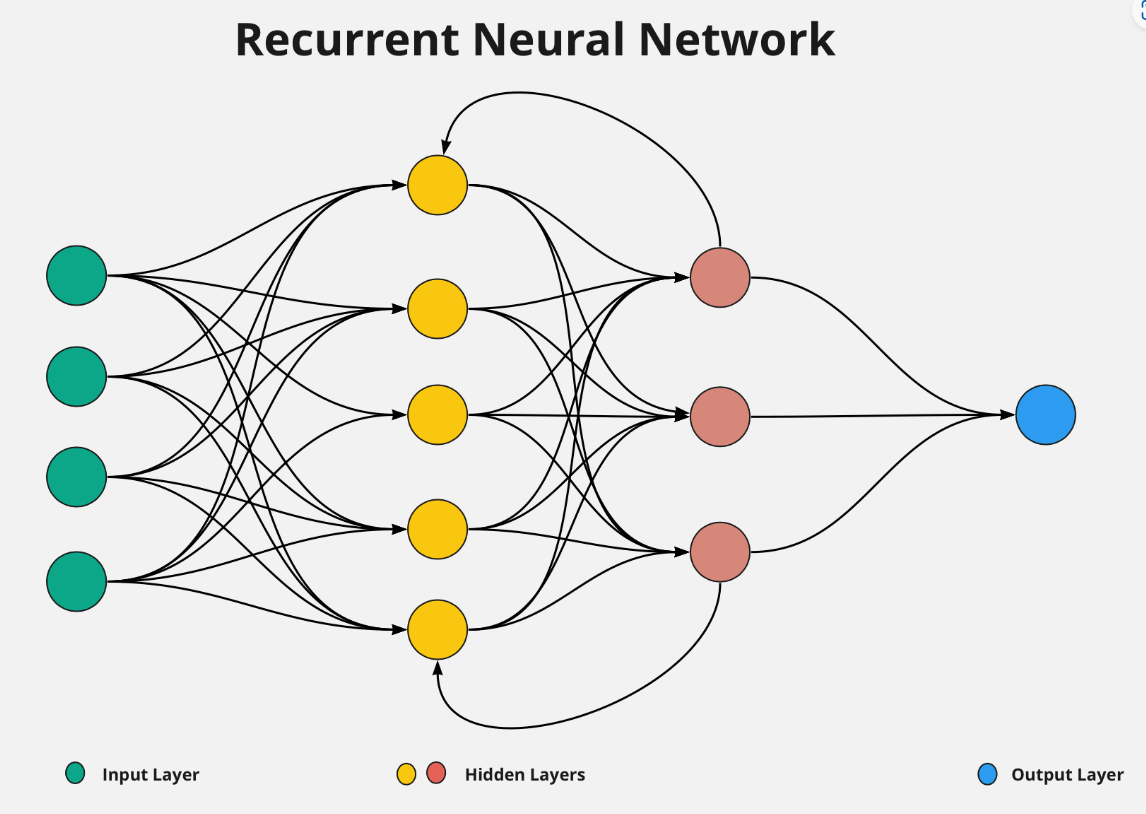
\includegraphics[height=4in,width= 4in ]{img/RNN.png}
    \caption{Recurrent Neural Network}
\end{figure}